\documentclass[a4paper,notitlepage]{article}
\usepackage{ssn-format}
\title{PFS ICS network connections}
\author{PFS ICS}
%\date{2014--08--06}
\begin{document}

\drafttrue
\SSNID{00002}
\SSNREV{003}
\SSNCATEGORY{ICS}
\SSNChangeRecord{
    Rev.2  / TUE-Opt stand-by, IR4(SpS) / 2014--08--06 \\ 
    Rev.1b / First Release (DRAFT rev.b) / 2014--01--22}
\SSNReference{(none)}
\SSNAttachment{(none)}
\SSNWritten{Atsushi Shimono}

\ssnhead

\section{Abstract}

This note contains ICD definitions on 
1) fiber assignment to PFS for communication, 
2) connection interface definition (media, format) for subsystems, 
and 3) network configuration diagram among PFS subsystems. 
Also overview of configuration at Subaru is included as an appendix 
for a reference and to have mutual understanding in the PFS. 


\section{Required connections for communication of subsystem}

In this section, external communication connections are listed per each 
subsystem. 

\subsection{PFI}

\subsubsection{USB over optical fiber / AG cameras}

PFI has 6 AG cameras controlled via USB 3.0, and we plan to pass USB 3.0 
to its control computer at CB2F via optical converter. 
PFS has selected PCI Express (PCIe) bus extender with optical fiber (SM) 
whose device board has a USB 3.0 controller, 
Part \# is Adnaco H1A (host) and R1USB30B (device) with SFP+. 

\subsubsection{MPS to positioner control}

MPS at CB2F communicates to FPGA board in PFI over ethernet by UDP. 
Assumed data flow rate is not so high, but RTT on communication is a key 
to control COBRA positioners. On this point, we are better to 
monitor and control using QoS, and are planning to use dedicated PFS-LAN 
but not shared E-LAN exists at Subaru. 

\subsubsection{Status monitoring and other control commands}

For status monitoring, including environment sensors and monitor hardwares, 
we need to have data connection from some control system to the control 
building, connected by ethernet. 

Monitoring (viewing) camera and microphone via USB audio will be 
connected via USB-Optical converter, and other sensors and controllers will be 
connedted to ethernet by AVR, PIC etc. 

\subsubsection{Cal lamp control}

Cal lamp for PFS is mounted over a cable wrapper on the PFI, control connection 
to the cal lamp controller need to be independent from the PFI. 
For this we need another fiber connection from CB2F for ethernet connection. 

\subsubsection{Summary}

PFI needs one pair of SM fiber for USB 3.0 exntension and two pair of 
fiber (MM or SM) for 1Gbps ethernet. 
For ethernet connection, PFS would like to have dedicated two pair of fiber 
connection available for PFS private network. 

Ethernet switch within PFI will be supplied by PFI team
\footnote{This is due to very limited space and power budget possible for 
control electronics and their cablse within PFI, and selection of network 
boxes need to be considered simultaneously with other mechanical parts and 
structure. SFP for this box will be supplied from IPMU which has verified 
connection over MM fibers at Subaru.}. 

\subsection{Cs / Metrology camera}

Metrology camera (CMOS sensor) will be controlled with computer in the Cs 
container for MCS, 
also we will add telemetry sensors and their controller. 
These control boxes will be connected directly to the ethernet. 
Required data rate is not high, since most largest is transferring acquired 
images to archive but not in real time. 

Ethernet switch at Cs is supplied by IPMU, an interface to 
each control box is a metal ethernet port (RJ45). 
One pair of fiber is required for 1Gbps ethernet between that switch and CB2F. 

\subsection{Spectrograph floor}

Due to assumed large data transfer volume and limited number of available 
fibers from SpS floor to control building (via NsIR patch panel), 
network plan and design from SpS floor to control building need to be 
flexible without mass impact to design of SpS floor. 
Therefore we designed SpS floor network in two separated stages: distribution 
switch to receive connection(s) from control building and to provide connection 
for SpS devices, internal metal ethernet of SpS devices. 
First stage between SpS distribution switch and CB2F is planned as FEC/LACP
\footnote{Link Aggregation Control Protocol (IEEE 802.3ad); PFS will not use 
PAgP. Planning to configure LACP load-balance as src-ip, but performance 
need to be verified by semi-real simulation, e.g. high traffic generation.}. 

Five identical racks are placed nearby SCR (Spectrograph Clean Room) at IR4, 
four racks are for four spectrograph modules (SM) which are identical each 
other, one rack (so called "fifth-rack") is for all other including SpS 
distribution switch. 

\subsubsection{Control for spectrograph module within SCR}

Control modules are mostly placed in the rack for each SM, except for three 
PC104 board computers and SAM for H4RG mounted on camera units. 
Each rack has one ethernet switch (as access layer) to accept RJ45 connection 
from SpS distribution switch, to provide network connection to devices and 
controllers. 

\paragraph{Camera control (PU/JHU)}

Each camera unit (xCU\footnote{BCU for blue, RCU for red, NCU for NIR}) 
outputs its acquired image and controls mechanics and thermal system 
within each camera (dewar): 

\begin{itemize}
  \item (BCU, RCU) CCD control and readout (BEE)
  \item (NCU) SAM (Sidecar Acquisition Module) for Teledyne H4RG control and readout
  \item PCM board, network switch and controller for sensors, serial communications and motors
  \item Vacuum ion pump (controller in the rack)
  \item Detector focus mechanism (three motors for each xCU)
  \item Cryocooler system (cryotel control, antivibe; 1 for BCU/RCU, 2 for NCU)
  \item Camera thermal control sensor
  \item Vacuum monitoring
\end{itemize}

Latter four systems are connected by serial or ethernet from PCM board, 
and external interface of PCM is one metal ethernet cable to a switch in the 
rack. 
Power modules and controllers for vacuum ion pump are mounted in the rack, 
and have connection to a switch in the same rack. 

BEE for CCD control and readout is CPU board + FPGA, and connects to 
a switch in the rack and MHS \footnote{An actor will run on this CPU board.} 
directly. 
No other control box will be required for BCU and RCU at SpS floor nor 
control building. 
Control and network connection to SAM for H4RG detector control is under 
investigation, one option is direct connection to metal ethernet under 
development but not succeeded yet, another option (used now) is USB control 
from BEE for NCU. For latter option, we might need to switch metal ethernet 
connection for BEE from a switch in the rack to SpS distribution switch. 
Since data flow rate for IR up-the-ramp readout will be 
around 300$\sim$500Mbps, and we transfer data to the control building directly 
from controller of SAM to save data into iSCSI storage at CB2F. 



\paragraph{Spectrograph module opt-mechanics control (LAM)}

Each spectrograph module has several movable opt-mechanics: 

\begin{itemize}
  \item Dithering mechanism
  \item Slit focusing mechanism
  \item Shutters (Blue, Red)
  \item Back illumination source
  \item Internal illumination source
  \item Red grating exchange mechanism
  \item Enviorment sensors (thermal, pressure, humidity etc.)
\end{itemize}

All controllers are mounted in the rack for each SM, and their network 
connections are connected within the rack. 


\subsubsection{Control hardware outside SCR}

\paragraph{SCR control and telemetry}

SCR thermal control and other telemetry devices are mounted in the "fifth-rack" 
and their network connections are connected to the SpS distribution switch. 

\paragraph{SpS infrastructure and other control devices}

Also as infrastructure items at SpS floor, following items are assumed, 
all will be connected to the SpS distribution switch: 

\begin{itemize}
  \item Fiber monitoring camera (by LNA)
  \item Surveillance camera (TBD: two in SCR, one outside SCR)
  \item PDU
  \item UPS (at IR3)
  \item Room light and air control sensor network
\end{itemize}

\subsubsection{Connection between CB2F and SpS}

Total network data rate is dominated by IR up-the-ramp readout which 
is assumed to be up-to $\sim$2Gbps for all four IR detectors, 
and other data flows including CCD readout are not high. 
Including mergin and possibility to separate network subnet, having four 1Gbps 
connections
\footnote{Several implementation plans are under discussion, but baseline is 
to keep at least 4Gbps in total. } 
would be safer. 

From only configuration point of view, we could take a way to have one fiber 
connections per each rack and five connections in total, considering number 
of available fibers and slots of SFPs at the core switch at CB2F, 
we decided to have four fiber 1Gbps connections between SpS distribution 
switch and the core switch in non-WDM
\footnote{Since fiber cables through the telescope structure were made 
at 1990's, these would be G.652 typed SM but not NS-DSF (need to be checked 
with initial specifications), using single core bidirectional mode will 
make risk on operation.}. 
Configuration of LACP need to be developed and verified before delivery to 
Subaru. 

\subsection{Summary of PFS communication over fiber}

PFS fiber communications are summarized as Figure.~\ref{fig:fiber-connection}. 

\begin{figure}[htb]
  \begin{center}
    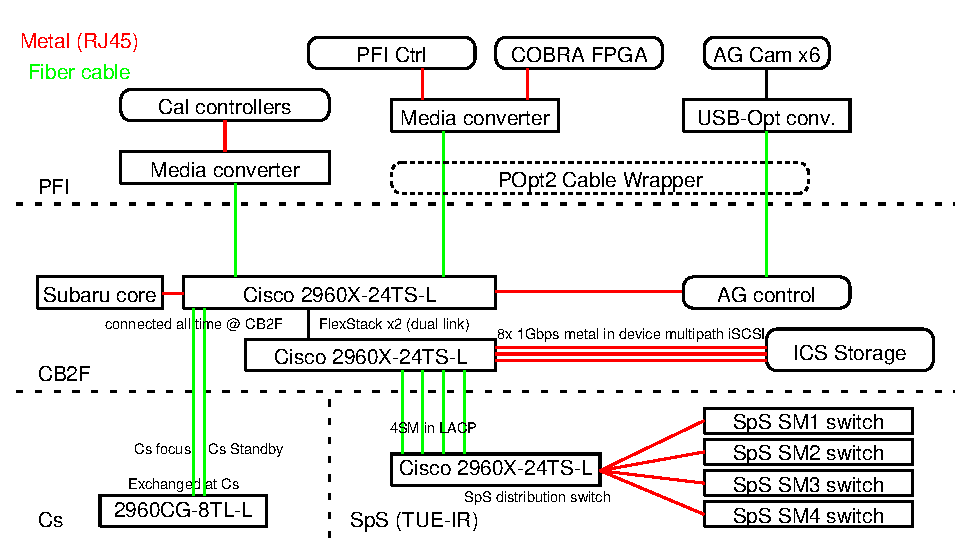
\includegraphics{networks-list.eps}
  \end{center}
  \caption{Schematic connection diagram for entire PFS fiber connections}
  \label{fig:fiber-connection}
\end{figure}


\section{Subaru fiber assignment}

\subsection{Request and Assignment}

Following items had requested to Subaru. 
All fibers are from control buidling patch panel. 

\begin{itemize}
  \item To have PFS dedicated ethernet network subnet (PFS-LAN)
  \item 1 pairs of SM fibers to PFI (PCIe optical extender for USB3)
  \item 2 pairs of MM (or SM) fibers to PFI (GbE)
  \item 4 pairs of SM fibers to SpS floor via NsIR (GbE)
  \item 1 pairs of SM or MM fibers to Cs (GbE)
  \item 1 pairs of SM or MM fibers to Cs Standby for PFS (GbE)
  \item 1 set of fibers to TUE (via NsOpt), same as a set to PFI
\end{itemize}

Assigned fibers by Subaru to the PFS are listed 
in Table.~\ref{tab:subaru-fiber}.
All cables are in MPO(4) connector, and have four fibers each. 

\begin{table}[htb]
\begin{center}
\caption{Assigned fibers by Subaru}
\label{tab:subaru-fiber}
\begin{tabular}{c|c|c|l}
to & fiber & mode & remarks \\
\hline
POpt2 & FB17401A & SM & at OCB21: A41J41-A41J42, A41J43-A41J44 (Spare) \\
POpt2 & FB17402A & SM & at OCB21: A41J45-A41J46 (Spare), A41J47-A41J48 (Spare) \\
POpt2 & FB17412C & MM 62.5 & at OCB21: A41J84-A41J83, A41J82-A41J81 (No spare) \\
\hline
TUE (NsOpt) & FB15305A & SM & 1 pair for spare \\
TUE (NsOpt) & FB15318C & MM 62.5 & No spare \\
\hline
SpS (NsIR) & FB15404A & SM & no spare \\
SpS (NsIR) & FB15405A & SM & No spare \\
\hline
Cs & FB14707A & SM & A1J81-84 (1 pair for Spare); Mostly to be assigned \\
Cs Standby & (FB13102A) & SM & Need to be tested and adjust auto connector position
\end{tabular}
\end{center}
\end{table}

\subsection{Test and fiber attenuation measurement results (2014/02)} 

\subsubsection{Fiber attenuation measurement method}

We could not prepare suitable calibration code or tail code since 
target connectors at patch panels were MPO, measurements were performed 
like 3-test code method or 1-test code method. 

We measured both patch cables + target and patch cables only. 
Connectors of target fibers are all MPO, we used MPO - 4x SC patch cable on 
each side. Laser outlets of SM/1310nm (CW) and MM/850nm are SC and directly 
connected to MPO-SCx4 patch cables, 
measurements' inlets could catch center cable guide (narrow stick w/fiber 
at its center) directly.
Measurement of patch cables + target are:
{\bf laser outlet - SC - MPO - (target) - MPO - SC - dBm measurement} 
and used MPO-MPO adopter for patch cables' measurement.
We did two measurements per each fiber connection, and rejected / re-measured 
when two have difference more than 1dBm. 
Fiber connectors of patch cables (MPO-SCx4) were cleaned before measurement, 
but we have not cleaned panel connectors. 

\subsubsection{Results}

Results of measurements are in Table.~\ref{tab:subaru-measurement}. 
Results for patch cables are subtracted. 

\begin{table}[htb]
\begin{center}
\caption{Measured fiber attenuations (dB)}
\label{tab:subaru-measurement}
\begin{tabular}{c|c|c||r|r|r|r||l}
to & fiber & mode & 1 & 2 & 3 & 4 & remarks \\
\hline
NsOpt & FB15315B & MM/50nm & 1 & 2 & 1 & 1 & Assigned \\
NsOpt & FB15318C & MM/62.5nm & 2 & 1 & 2 & 2 & Assigned \\
NsOpt & FB15319C & MM/62.5nm & 1 & 2 & 2 & 2 & \\
NsOpt & FB15320C & MM/62.5nm & 2 & 1 & 2 & 2 & \\
NsIR & FB15404A & SM & 2.0 & 3.0 & 2.5 & 2.4 & Assigned \\
NsIR & FB15405A & SM & 0.2 & 1.1 & 0.9 & 1.9 & Assigned (Measured by Matt-san) \\
NsIR & FB15406A & SM & 1.6 & 0.9 & 1.9 & 18.4 & \\
NsIR & FB15408A & SM & 1.5 & 0.5 & 2.5 & 1.4 &  \\
NsIR & FB15409A & SM & 1.7 & 1.7 & 3.3 & 1.8 &  \\
NsIR & FB15410A & SM & 0.6 & 1.1 & 1.1 & 0.9 &  \\
\end{tabular}
\end{center}
\end{table}

\appendix

\section{Overview of Subaru networks}

We need to care of two items to distinguish "network" at Subaru, one is 
cable IDs for wire (or outlet IDs at patch panel) 
and another is network IDs for L3 layer. 
For our network connection among subsystem places (e.g. control building, 
PFI, Cs, SpS), we will use fiber cables for wire
\footnote{We can get metal/TP by attaching media converter, but every 
connection will be fiber at patch panel.}. 

This section overviews these available networks at Subaru. 

\subsection{Fiber cables}

From control building (computer room at 2nd floor) to each focus in the 
Subaru dome, we will use fiber cables to connect our subsystems onto network. 

Fiber cables are labeled as FBxxxxxY, where x is digit and Y is A/B/C, 
each ID is not for a single fiber but for a set of fiber and number is not 
fixed. Number of fibers in one ID depends on its connector, like 4 fibers for 
MPO(4), or 2 fibers for SC Duplex. 
5-digit number is an unique ID for the cable, A/B/C is a specification of 
"fiber cable" but not for connector at patch panel each side
\footnote{Different fiber connector could be used for two ends.}.
Mostly the same ID is used for label of two connectors at patch panel for both 
ends, at some ports (e.g. junction boxes or terminals on the telescope) 
connector is labelled as AxJy, where x is terminal number and y is 
connector ID in the terminal, with x or y in multi-digit ID. 

\begin{description}
  \item[A] SM 9.5 um
  \item[B] MM/GI 50 um 
  \item[C] MM/GI 62.5 um
\end{description}

\subsection{Networks}

Existing Subaru networks are marked as X-LAN or X-LAN(Y), like V-LAN or 
E-LAN(C), and each network is defined as one "subnet" with class C private 
network. 
For E-LAN(x) networks, originally these are defined by target application 
and its required network speed (at 1990s...), but these are just subnet 
definitions as for now. 
Following is a (subset) list of available networks: 

\begin{description}
  \item[E-LAN(C)] was defined as "control" network, connected to dome by 10B 
    (metal-optical converter)
  \item[E-LAN(D)] was defined as "data" network, connected to dome by 100B 
    (metal-optical converter)
  \item[E-LAN(G1)] was defined as "gigabit" network, directly connected to 
    each instrument or network in dome
  \item[E-LAN(G2)] was defined as "gigabit" network, directly connected to 
    dome (seems to be added for increasing IP address??)
  \item[V-LAN] Video network for real time display (e.g. AG image),
    using pre-formatted RPC (connected to VGW system)
\end{description}


\end{document}

